%% LyX 2.3.0 created this file.  For more info, see http://www.lyx.org/.
%% Do not edit unless you really know what you are doing.
\documentclass[12pt,english]{article}
\usepackage{mathptmx}
\usepackage[T1]{fontenc}
\usepackage[utf8]{inputenc}
\usepackage{geometry}
\geometry{verbose,tmargin=1in,bmargin=1in,lmargin=1in,rmargin=1in}
\setcounter{secnumdepth}{2}
\setcounter{tocdepth}{-2}
\usepackage{float}
\usepackage{amsmath}
\usepackage{graphicx}
\usepackage{setspace}
\usepackage[authoryear]{natbib}
\usepackage{multirow}
\doublespacing

\makeatletter
%%%%%%%%%%%%%%%%%%%%%%%%%%%%%% User specified LaTeX commands.
\usepackage{dcolumn}
%\usepackage{indentfirst}
\usepackage{parskip}
\usepackage{booktabs}
\date{}
%\usepackage{endnotes}
%\let\footnote=\endnote
\usepackage{graphicx}
\newcommand{\indep}{\rotatebox[origin=c]{90}{$\models$}}
\renewcommand\thesection{\Roman{section}}
\renewcommand\thesubsection{\Alph{subsection}}
%\usepackage{tikz}  % main function for plotting game
%\usetikzlibrary{calc}  % calculations of coordinates
%\usetikzlibrary{arrows, automata}% LaTeX
%\usepackage{rotating}
\usepackage[ragged, bottom, multiple]{footmisc}
\usepackage[colorlinks, urlcolor=blue, citecolor=blue, linkcolor=blue]{hyperref}

\@ifundefined{showcaptionsetup}{}{%
 \PassOptionsToPackage{caption=false}{subfig}}
\usepackage{subfig}
\makeatother

\usepackage{babel}
\begin{document}
\begin{spacing}{1}

\title{\textbf{Who's in Charge, Who Do I Work With, and Who Are My Friends:
A Latent Space Approach to Understanding Elite Coappearances in China}\thanks{The replication datasets and codes will be available online.}}
\maketitle
\begin{abstract}
\begin{flushleft}

How the ruling elite arrange and maintain their power-sharing is key
to our understanding of authoritarian politics. We propose a latent
space framework to systematically analyze the dynamics of elite power-sharing
in authoritarian regimes. We also introduce a novel dataset tracking
appearances of elite Chinese Community Party (CCP) members at political
events. Our new framework and data allow us to disentangle three key
aspects of elite power-sharing in authoritarian regimes: (1) who's
in charge, (2) who do I work with, and (3) who are my friends. We
empirically assess the three questions by computing elites' total
appearances, dyadic coappearances, and their latent network distance
using a latent factor network analysis of about 10000 appearance records
of over 200 top CCP elites from 2013 to 2017. We test how well these
three indicators fare in predicting elites’ appointments in the leading
small groups (LSGs) of the CCP Central Committee and the Central Government.

\end{flushleft}
\end{abstract}
\end{spacing}

\newpage{}

%\clearpage
%\setcounter{page}{1}
\renewcommand{\footnotesize}{\normalsize}
\renewcommand{\footnotelayout}{\raggedright\doublespacing} % set spacing in footnotes
    \newlength{\myfootnotesep}
    \setlength{\myfootnotesep}{\baselineskip}
    \addtolength{\myfootnotesep}{-\footnotesep}
    \setlength{\footnotesep}{\myfootnotesep} % set spacing between footnotes 
\begin{flushleft}
\setlength{\parindent}{2em}
\setlength{\parskip}{0pt}

Only one in ten autocrats are toppled down by popular uprisings. Most
authoritarian rulers are instead ousted by regime insiders \citep{Svolik2012}.
How the ruling elite arrange and maintain their power-sharing is thus
key to our understanding of authoritarian politics \citep{BDMetal2003,Acemoglu2008a,Svolik2012}.
A burgeoning literature turns to authoritarian institutions (e.g.,
national legislatures) and explores how institutionalization of power-sharing
contributes to authoritarian resilience \citep[e.g,][]{Brownlee2007,Gandhi2008,Magaloni2008,Magaloni2010,Boix2013a},
as well as economic growth \citep[e.g.,][]{Bizzarro2018}, social
welfare provision \citep[e.g,][]{Miller2015b}, and accountable foreign
polices \citep[e.g.,][]{Weeks2012}. However, as stressed by \citet{Pepinsky2014},
a fundamental dilemma confronting this ``institutional turn'' is
that these institutions are inherently endogenous to strategic interactions
of the ruling elite (also see \citealp{Brancati2014a}). That is,
de facto cooperation and contention of the authoritarian elite still
hide behind the facade of formal institutions.

Another group of scholars have adopted an alternative and elite-oriented
approach to uncovering the inner workings of authoritarian regimes.
Relying on a wide range of data like anecdotes, interviews, media
coverage, and biographical archives, these studies try to identify
key elites and analyze their social backgrounds, career patterns,
and patronage ties \citep[e.g.,][]{Li1989,Levitsky2001,Albrecht2004,Perthes2004,Shih2010,Opper2015,Buehler2017}.
However, partly due to data limitations, we find few attempts to synthesize
different aspects of elite dynamics, leaving us with only a fragmented
perspective on power-sharing in authoritarian regimes. Unfortunately,
it is this lack of a systematic approach that fundamentally constrains
our understanding of authoritarian politics.

In this article, we propose a latent space framework to systematically
map and analyze the dynamics of elite power-sharing in authoritarian
regimes.\footnote{To clarify, here we use the term of latent space in a generic sense,
i.e., some area where elites with similar preference are in proximity
to each other. In our later analysis, we treat the space as a latent
factor space and use the the Latent Factor Model \citep{Hoff2005,Minhas2016a},
which is different from the Latent Space Model proposed by \citet{Hoff2002}.} We also introduce a new type of data that has yet to come to attention
of scholars of authoritarian politics, that is, elite appearance and
coappearance at political events. Our new framework and data allow
us to disentangle and synthesize three key aspects of elite power-sharing
in authoritarian regimes: (1) who's in charge, (2) who do I work with,
and (3) who are my friends. The question of ``who's in charge''
focuses on the power and influence of \emph{individual} elites. The
answer to this question is of critical importance in authoritarian
regimes where formal political institutions are vulnerable to elites'
manipulation. Moving beyond individual and monadic elites, the question
of ``who do I work with'' points to the \emph{dyadic} relationship
between a given pair of elites (e.g., collegial ties and patronage
connections), which serves as the very basis of coalitions and factions.
However, a simple dyadic ``who do I work with'' approach will, we
argue, overlook the indirect and latent relationships between elites
and forgo important information about latent coalitions. For instance,
without a direct collegial or patronage connection, two elites could
still form a latent coalition because of their ties to a common friend.
The question of ``who are my friends'' then captures such indirect
\emph{latent} connections between elites. Together, by jointly considering
the monadic, dyadic, and latent attributes, the three ``who'' questions
reveal systematic dynamics of elite power-sharing in authoritarian
regimes.

Our empirical analyses and tests are focused on the Chinese Communist
Party (CCP) regime. While the CCP regime has been commonly accepted
as one of the most institutionalized and ``machine-like'' authoritarian
regimes, many China scholars emphasize that institutional rules are
epiphenomenal to elite politics \citep{Nathan1973,Tsou1976,Shih2010}.
After Xi Jinping became the general secretary of CCP in 2012, the
interest in elite power-sharing has been rekindled and become even
more heated. Xi's first term was marked with major elite reshuffles,
swift institutional changes, and wide-ranging policy alterations \citep{Miller2014b,Naughton2014,Lampton2015,Shirk2018}.
These dramatic changes not only urge us to reassess CCP's intra-elite
relations, but also make it an ideal laboratory to explore the three
``who'' questions. Specifically, we utilize a latent factor network
model \citep{Minhas2016a} and analyze a unique database that tracks
about 10000 appearance records of over 200 top CCP elites from 2013
to 2017. We attempt to answer the three ``who'' questions by computing
elites' total appearances (i.e., ``who's in charge''), dyadic coappearances
(i.e., ``who do I work with''), and, finally, their latent network
distance (i.e., ``who are my friends''). Together, our latent factor
analysis of the appearance data presents a possible avenue to disentangle
and synthesize key aspects of elite power-sharing in authoritarian
regimes.

To probe the validity of this approach, we examine how well these
three indicators fare in generating out of sample predictions of elites'
appointments in the leading small groups (LSGs) of the CCP Central
Committee and the Central Government \citep{Batke2017,Huhe2018a}.
LSGs are an informal institutional arrangement of CCP that has not
been incorporated into charts of party or government organs. However,
they play a pivotal role in formulating, coordinating, and implementing
of important decisions across different segments and levels of the
CCP regime \citep{Hamrin1992,Lieberthal1992a}. LSGs not only ameliorate
the regime's prolonged problem of political fragmentation, they can
also be an effective vehicle for overpassing formal institutions and
asserting personal influences as shown by the infamous Central Cultural
Revolution Group (1966-69). Recently, it has been found that Xi relied
heavily on LSGs to push forward institutional reforms and policy changes
\citep{Miller2014a,Naughton2014,Johnson2017,Lee2017,Shirk2018}. Our
tests then show that while elites' total appearances are strongly
associated with their appointments in LSGs memberships, their dyadic
coappearances bear a much weaker association. Most notably, the best
predictor of LSG membership is our latent measure of network proximity.

Our study contributes to the extant studies of authoritarian politics
in many ways. First, our latent space framework (i.e., the three ``who''
questions) provides a possible approach to bridge and synthesize the
fragmented studies of the ruling elite in authoritarian regimes. This
allows us to develop a systematic assessment of their power-sharing
patterns and dynamics. Second, our approach explicitly highlights
and models the latent relationships between elites, which so far has
received only scant scholarly attention. As revealed in our analysis
of LSG appointments, the incorporation of such latent distances could
significantly improve our assessment about elite power-sharing. Finally,
our study introduces a new source of data, i.e., public appearances
of the elite. The appearance data not only complements our existing
data like news coverage and biographical archives, but, more importantly,
allows for a systematic exploration of the dynamic and relational
changes in elite power-sharing.

\section*{Literature Review: The Elite and Their Relationships}

How to understand the elite and their relationships behind the facade
of formal institutions has been one enduring question in social science.
For instance, the ``power elite'' thesis emerged in 1950s stimulated
a heated debate on whether power in America was concentrated on a
small cohesive group of quasi-hereditary and well-positioned elites
\citep{Hunter1953,Mills2000,Dahl1961}. The debate in turn has significantly
advanced our understanding about the nature of democracy \citep[e.g.,][]{Dahl1971}.
In studies of authoritarian politics, scholars have been increasingly
confronted by the same problem, particularly after the recent development
in studies of authoritarian institutions. Although recent theoretical
works like \citet{Svolik2012} provide us valuable insights to link
authoritarian institutions with elite contention and cooperation,
we still lack a systematic framework to conceptualize and analyze
the actual power-sharing dynamics in authoritarian regimes.

Our lack of a systematic framework has much to do with the highly
secretive nature of authoritarian politics. It restricts researchers
to employing methods such as Hunter's \citeyearpar{Hunter1953} sociometric
interviews using ``power elite'' debates. Many studies of authoritarian
elites, therefore, have ``been based on anecdotal and impressionistic
`readings of the tea leaves'{}'' \citep[p. 137]{Ishiyama2014}. Given
these limitations, a number of scholars have introduced novel empirical
approaches to explore different aspects of elite politics. Such studies
are particularly developed in the studies of the CCP elite, and they
largely fall into two separate lines of inquiries: (1) identifying
key actors (i.e., the positional approach) and (2) exploring their
relations (i.e., the relational approach).

First, the positional approach focuses on \emph{individual} elites
and aims to assess their de facto positions within the CCP regimes.
\citet{Jaros2017} exemplifies this approach as they explore Xi's
actual power and influence by examining CCP's official newspaper coverage.
It is argued that the ruling elite usually rely on official media
to signal their political presence and influence to the lower-level
officials and the general public \citep{Huang2015b}. Their coverage
in official newspapers, therefore, can be used to infer their ability
to dominate the party-state. Based on their collection and analysis
of province-level party newspapers between 2011 and 2014, \citet{Jaros2017}
find that Xi has received disproportionately more coverage over time,
indicating a consolidating grip on power. Such large-scale quantitative
analysis of texts allow us to reveal ups and downs of key elites in
a dynamic way.\footnote{For similar studies, see the review of \citet{Ban2018}.}
However, due to its focus on individual elites, this approach falls
short in uncovering the relations between CCP elites.

The relational approach, on the other hand, examines \emph{dyadic}
affinity and ties between elites. This empirical approach is rested
on the thesis of factional politics. It postulates that the political
struggle between competing factions is the key to our understanding
of CCP elite politics, and a faction usually grows out of patron-client
relationships that are cultivated by a patron through the career path
\citep{Pye1981,Nathan1995,Huang2000,Shih2010,Shih2012}. Empirically,
scholars rely on biographical archives to uncover such patron-client
relationships. Based an extensive review, \citet{Meyer2016} identify
four different empirical indicators of factional ties, i.e., broad
ties, complete work ties, early work ties, and restrictive work ties.
They further examine how CCP elites' varying ties with the party secretary
general predict their promotion into the Central Committee. Their
analysis shows that while work ties with the secretary general consistently
matter, non-work ties (e.g., a common educational background) sometimes
could also help. In light of this, by steering our attention to factional
ties associated with key patrons, this approach helps us to move beyond
the power core and probe links across ruling elites.

While these two approaches provide us important insights about elite
dynamics of the CCP regime, we find that some critical problems remain
unresolved. First and foremost, we still lack a conceptual framework
to synthesize different insights from the existing studies (e.g.,
dynamic changes of personal powers on the one hand and abiding factional
ties between patrons and clients on the other). This in turn hinders
our systematic understanding of elite power-sharing. Second and more
specifically, our emphasis on key patrons and their direct clients
tend to leave much valuable information neglected. This is mainly
due to the importance and prevalence of \emph{indirect} and \emph{non-dyadic}
relationships. A client of a factional leader, for instance, could
also serve as the patron for other elites, forming a three-party relationship.
The existence of such indirect relationships not only significantly
increases the scope of factions, but, more importantly, generates
a complex interdependent network of elites. Without a systemic study
of such indirect relationships, we are unable to answer a series of
important questions like hierarchies within factions or nuanced distinctions
between apathetic and antagonistic relationships. Thus by using extant
approaches, we are limited to only looking at direct relationships
rather than being able to holistically study the complete system of
affinity, patronage, and antipathy. To understand elite dynamics,
and thus authoritarian politics writ large, requires both new conceptual
exploration and empirical strategies.

\section*{Elite Power-Sharing as a Latent Space}

In this study, we conceptualize the elite power-sharing in authoritarian
regimes as a latent space. This latent space not only encompasses
a collection of individual elites, it subsumes all the relationships
between them, direct or indirect. In light of this, a latent space
understanding could allow us to synthesize both \emph{positional}
and \emph{relational} attributes of the ruling elite and thus develop
a systematic view about power-sharing in authoritarian regime. Yet,
despite its apparent conceptual advantages, a latent space understanding
requires us to answer two critical questions: (1) how to capture it
and (2) how to analyze it.

\subsection{Political Events and Power \emph{Foci}}

How to capture the power elite and their relationship has been a key
front of the power elite debate \citep{Domhoff2005}. In \emph{Who
Governs? Democracy and Power in an American City} \citeyearpar{Dahl1961},
Dahl argues that the problem has risen from the obscure distinction
between the legal theories of power and the realities of power: ``the
American creed of democracy and equality prescribes many forms and
procedures from which the actual practices of leaders diverge. Consequently,
to gain legitimacy for their actions leaders frequently surround their
covert behavior with democratic rituals'' (p. 89). Recognizing this,
Dahl proposes to focus on political events and meetings where the
actual processes of influence are at work. For instance, after observing
local political nominations, Dahl finds that ``the number of persons
who have participated in these decisive negotiations and influenced
the outcome seems never to have been more than a half dozen in recent
years'' (p. 105). 

In this study, we follow Dahl's approach and turn to what we call
power \emph{foci}, i.e., important political events and meetings as
well as elites' appearances at them. The concept of foci is originally
introduced by \citet{Feld1981} to explore people's complex and embedded
social circles in a community. A focus is usually defined as a social
entity or event around which joint activities are organized (e.g.,
voluntary organizations, hangouts, and families). Since it is around
these foci that individuals organize their social relations, we could
learn essential features of their latent social space by studying
the observable foci. Similarly, we argue that political events like
ceremonies, policy meetings, and state visits can be treated as power
foci, around which the ruling elite signal and manage their power
relationships. For instance, an elite's presence in a policy meeting
would suggest her or his involvement in the decision-making activities
and thus convey valuable information about the actual processes of
influence. As the ruling elite coordinate with each other via numerous
such events, we could approximate their latent space of power-sharing
by examining how these foci are interconnected.

The interlocking network of power foci reveals both positional and
relational attributes about the ruling elite. It is positional in
its ability to uncover individual elites' relative activeness and
prominence in events where the actual processes of influence are at
work. Moreover, the particular patterning of an elite's appearance
defines her or his points of reference in the nebulous ruling group.
This is consistent with Dahl's \citeyearpar{Dahl1961} emphasis on
observing decision-making activities. The interlocking foci network
is also relational. Beyond specific events or individual elites, it
shows how elites are connected via a variety of political events.
Political elites intersect with each other within different political
events, which are created based on shared policy problems or personal
affinities. These links are not only able to channel important resources
like information, but also can support mechanisms through which elites
monitor and sanction each other.

\subsection{Three ``Who'' Questions in a Latent Space}

So how can we approximate the latent space of power-sharing from the
interlocking foci network? In this study, we treat the foci network
as a product of both stochastic and strategic factors. We further
disaggregate the strategic factors into three questions --- i.e.,
who's in charge, who do I work with, and who are my friends, which
correspond to the individual level characteristics, dyadic links,
and latent affinities. Generally speaking, our approach can be summarized
as follows: after controlling for random noise, powerful elites (i.e.,
who's in charge) are more likely to make appearances; elites who are
in the same and related policy domains (i.e., who do I work with)
are more likely to appear together; and finally elites who share latent
affinities (i.e., who are my friends) are more likely to show up together.
Together, the 'three' who questions help us to approximate the latent
space of elite power-sharing.

The first two who questions are quite consistent with the existing
studies of elite politics. Similar to such positional studies as \citet{Jaros2017},
the question of who's in charge is focused on network dynamics that
are stemmed from characteristics of individual elites. For instance,
certain type of actors tend to be more active in initiating connections.
In our case of elite politics, this suggests that powerful elites
are more likely to preside and participate in important ceremonies
and meetings. From the network analysis perspective, this greater
tendency of certain actors to undertake certain behaviors is usually
referred as the first-order dependency \citep{Hoff2005,Kenny2006}.
In light of this, we expect, for example, Xi Jinping is simply going
to make more appearances in aggregate than would a junior CCP elite.
That is, if we compare two possible elites, a third person is \emph{ceteris
paribus} more likely to make a coappearance with Xi than with the
junior CCP elite. On the other hand, the second who question examines
if two elites attend the same event. Given its focus on the observable
direct and dyadic links, this question follows the similar approach
like \citet{Shih2010}. The question of ``who do I work with'' then
highlights whether there is a direct coordination and collaboration
between a pair of elites. 

However, what we emphasize in this study is that we cannot equate
``who do I work with'' with ``who are my friends.'' Simply using
direct and dyadic links as a proxy of the latent affinity could lead
to two types of errors, the incorrect rejection of a true friend and
the false acceptance of a real enemy. A simply example of the first
error is an indirect patronage relationship which involves a patron,
a client, and a sub-client. If we rely solely on dyadic coappearance,
we may end up in wrongly rejecting the relationship between the patron
and sub-client. The second error could also occur in a three-party
relationship when an elite share links with two rival patrons. In
this case, we could run into either a false conclusion or no conclusion
at all. Provided with these possible errors, some scholars have questioned
the validity of factional studies based on dyadic analyses. For example,
\citet{Miller2015d}, a long-time observer of CCP elite politics,
points to two problematic cases (i.e., Liu Yunshan and Li Yuanzhao),
both of whom share strong ties with competing Jiang and Hu factions.
Without a consistent criterion, she argues that ``in the Xi era,
faction-based analyses frequently rest on assertions of factional
association that are tenuous, arbitrary, and at times peculiarly fungible''
(p. 7).

In this study, we argue that the above problems stem from the prevalence
of indirect ties in elite politics, and one remedy is to examine the
more complex and non-dyadic relationships like the aforementioned
three-party transitivity problems. We thus turn to the question of
``who are my friends,'' which is commonly accepted as the third
order dependency in network analysis.\footnote{The second-order dependency usually refers to reciprocity, which does
not apply to our case here.} Unlike first-order dependencies that are associated with attributes
of individual actors, such high-dimensional dependencies usually arise
from mechanisms like homophily and stochastic equivalence. Homophily
is the tendency for actors who share unobserved characteristics, for
example their patron-client linkages, are more likely to be linked
and make coappearances than actors that do not share those characteristics.
Stochastic equivalence is the idea that actors might have similar
roles in the network, and thus be more or less likely to make appearances
with common coalitions. If two elites in China are both proteges of
Xi Jinping, then they are both more likely to make co-appearances
with Xi and his other proteges, and less likely to make co-appearances
with Xi's rivals and his rivals' proteges. Therefore, a systematic
study of such indirect ties helps us to understand the complex interdependencies
between elites and thus provides a more accurate answer to the question
of ``who are my friends.''

\vspace{24bp}

To sum up, in this study we propose to conceptualize the elite power-sharing
as a latent space, which allows us to synthesize both of its positional
attributes and relational dynamics. We further argue that we can approximate
this latent space by examining how power foci (i.e., political events
and elites' appearance at them) are interconnected. Finally, we highlight
the three who questions we need to answer in this approximation. In
the following parts, we introduce our empirical strategies and discuss
how the approach could help shed light on the development of such
informal institutions as LSGs.

\section*{Data}

In this study, we rely on a unique database from the China Vitae project,
which tracks the public appearances of the CCP elites. We focus on
the time period between January 1 2013 and January 1 2017, and there
are about 10,000 appearance records of over 200 elites. This allows
us to systematically examine the elite power-sharing in Xi's first
term. Table 1 presents a small sample of our dataset and reports the
date, the event, and elites in attendance.\footnote{Further information about the event locations, topics raised, and
sources are also available.} From Table 1, we can find our dataset captures how top CCP elites
structured their power relationships via a variety of political activities,
ranging from the civil-military unity meeting to the China-US summit.
As argued above, these power foci constitute an interlocking network
of events and elites, and Figure 1.a shows how the six sample events
in Table 1 could form a simple interlocking network. Since our main
focus is elite relationships, we then extract the elite coappearance
network as shown in Figure 1.b, and this coappearance network serves
as the starting point of our later analyses.

\noindent \begin{center}
\begin{table}[H]
\caption{A selected sample of political events}

\centering
\small
\begin{tabular}{p{1in}p{3in}p{2in}}
  \\[-1.8ex]\hline
  \hline \\[-1.8ex]
   Date & Event & Attendee \\    \hline \\[-1.8ex]

  \tt{2013-01-25}  & \tt{Vice-Chairman of the Central Military Commission calls for efforts to promote unity among army, government and the people} & \tt{Zhang Gaoli, Xu Qiliang}\\
    &  &  \\
  \tt{2013-02-07}  & \tt{Xi Jinping urges \#CPC to accept criticism and be receptive to the views of non-communists} & \tt{Xi Jinping, Li Keqing, Yu Zhengsheng}\\
    &  &  \\
   \tt{2013-03-18}  & \tt{Xi Jinping endorses work of Hong Kong \#HK, \#Macao governments \#China} & \tt{Xi Jinping, Zhang Dejiang, Li Yuanchao, Yang Jiechi}\\
    &  &  \\
   \tt{2013-04-14}  & \tt{Premier stresses foresight in economic policymaking \#China} & \tt{Li Keqiang, Zhang Gaoli, Ma Kai, Liu Yandong}\\
    &  &  \\
   \tt{2013-05-20}  & \tt{Chinese Premier visits memorial of Mahatma Gandhi in New Delhi \#India \#China} & \tt{Li Keqiang, Wang Yi}\\
    &  &  \\
   \tt{2013-06-07}  & \tt{Xi, Obama meet for 1st summit \#China \#USA} & \tt{Xi Jinping, Wang Yi}\\
   ... & ...  & ... \\ \\[-1.8ex]     \hline 
 \hline \\[-1.8ex]
\end{tabular} 
\end{table}
\par\end{center}

\noindent \begin{center}
\begin{figure}[H]
\noindent \begin{centering}
\subfloat[]{\noindent \begin{centering}
\includegraphics[width=2.5in]{figure/data_fig1}
\par\end{centering}
}\subfloat[]{\noindent \begin{centering}
\includegraphics[width=2.5in]{figure/data_fig2}
\par\end{centering}
}
\par\end{centering}
\caption{The interlocking networks of power foci}
\end{figure}
\par\end{center}


\noindent \begin{center}
\begin{figure}[H]
\noindent \begin{centering}
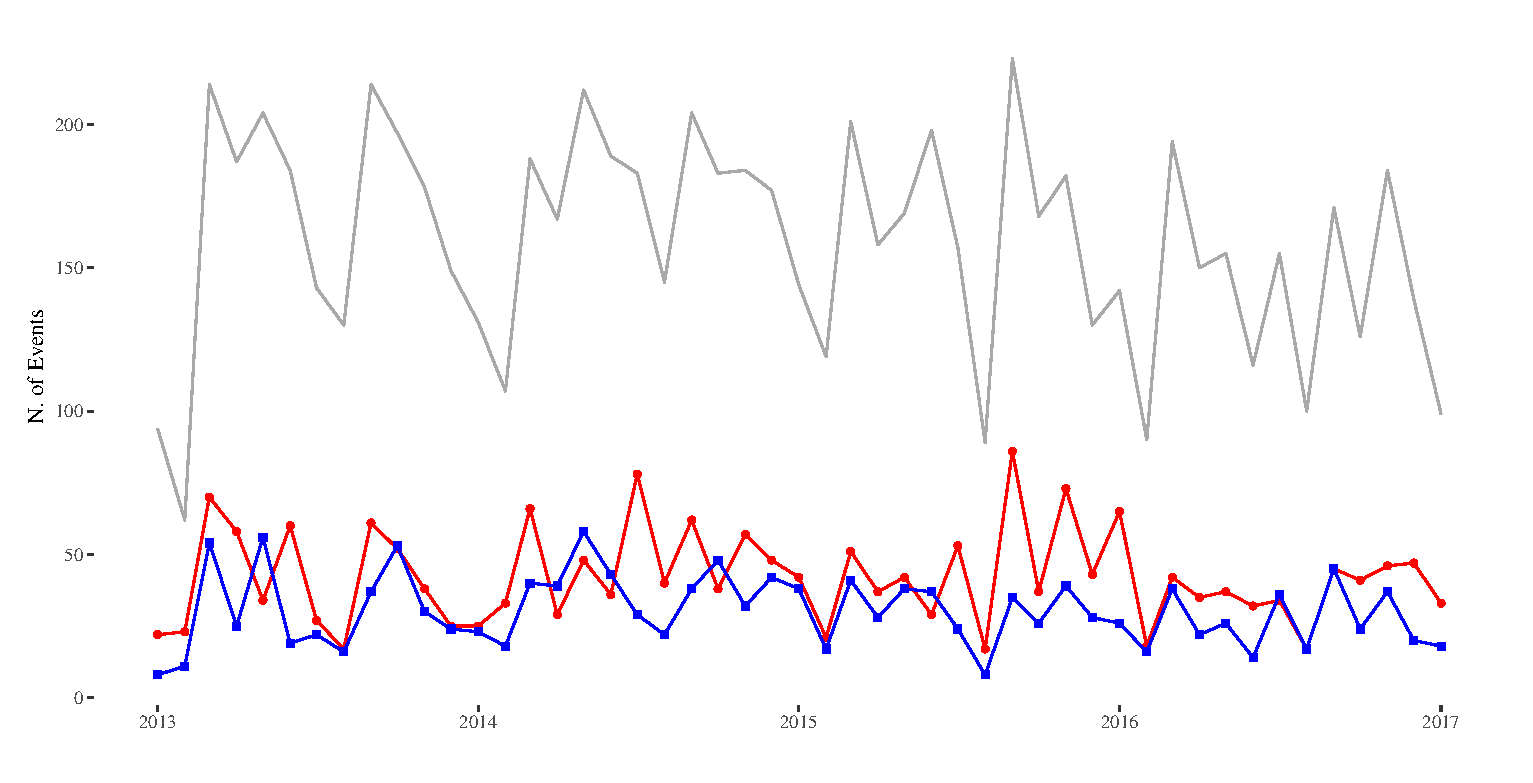
\includegraphics[width=5in]{figure/freq}
\par\end{centering}
\caption{Total appearances (gray), Xi (red), and Li (blue)}
\end{figure}
\par\end{center}

After constructing the complete coappearance network, we can answer
the questions of ``who's in change'' and ``who do I work with''
by calculating elites' total appearances and coappearances. Figure
2 plots the total number of elite appearances (gray), as well as those
associated with Xi Jinping (red) and Li Keqiang (blue) respectively.
A quick examination shows a consistent annual pattern. There are much
fewer elite appearances in February and August, and their activities
peak in March and September. While the low points in springs are mainly
due to the Chinese new year, those in August have a lot to do with
the CCP's tradition of Beidaihe retreat \citet{Miller2014c}. A comparison
of Xi and Li's appearances points to some interesting changes. In
2013 and 2014, we can find that their total appearances frequently
intersected. Yet starting from 2015 Xi has made markedly more appearances.
This corroborates with \citet{Jaros2017} that Xi has significantly
consolidated his power in his first term.
\noindent \begin{center}
\begin{figure}[H]
\noindent \begin{centering}
\subfloat[Xi and Li]{\noindent \begin{centering}
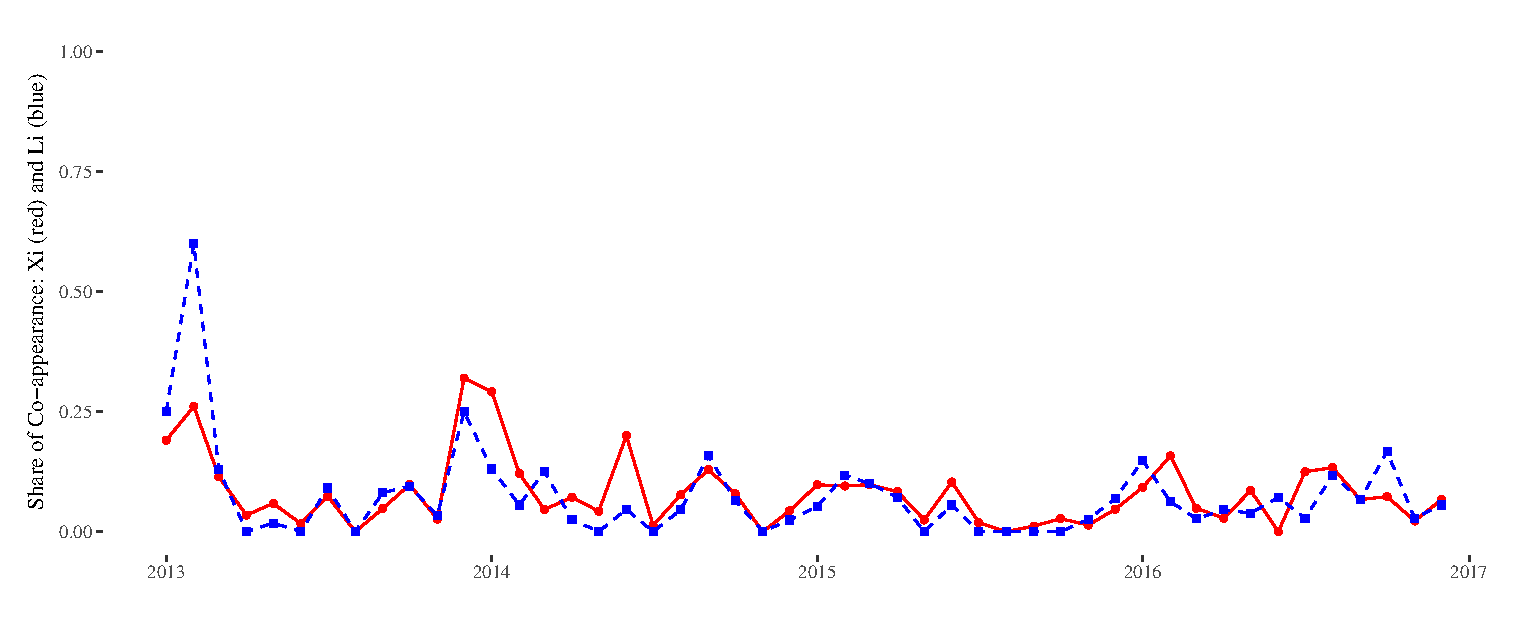
\includegraphics[width=5in]{figure/Xi_Li}
\par\end{centering}
}
\par\end{centering}
\noindent \begin{centering}
\subfloat[Xi and Zhang]{\noindent \begin{centering}
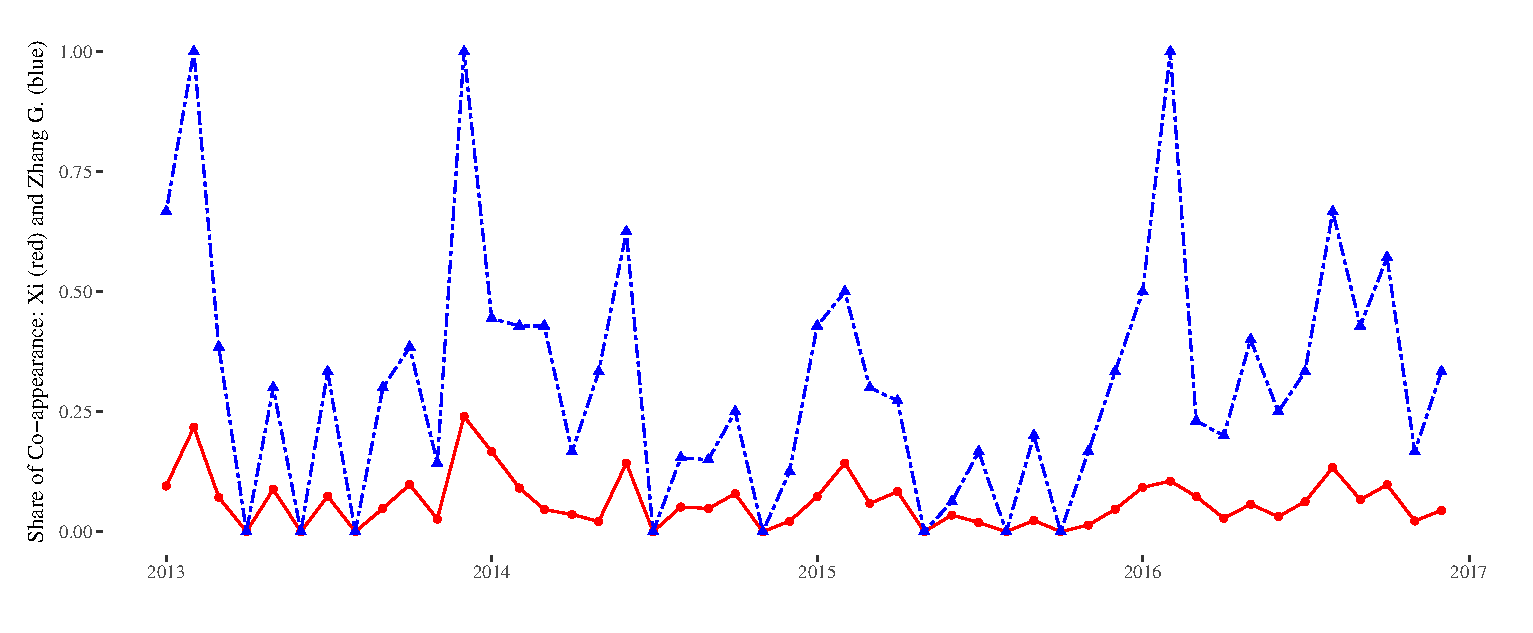
\includegraphics[width=5in]{figure/Xi_ZG}
\par\end{centering}
}
\par\end{centering}
\caption{Coappearance}
\end{figure}
\par\end{center}

In Figure 3, we plot and contrast two pairs of coappearances, Xi-Li
and Xi-Zhang.\footnote{Zhang Gaoli was one of the seven members of the Politburo Standing
Committee, who also served as the first-ranked Vice Premier.} In Figure 3a, while the red line indicates the share of Xi-Li coappearance
to Xi's total appearance, and the dashed blue line denotes the share
of their coappearance to Li's. From Figure 3.a, we can find that the
two lines intersected throughout the four years, and their shares
of coappearances have declined over time. In other words, for both
Xi and Li, their coappearances account for similar weights in their
total activities, though they were gradually departing away from each
other. However, Xi-Zhang coappearances in Figure 2b show a different
trend. Xi-Zhang coappearances were highly asymmetrical. The share
of their coappearance is markedly more salient for Zhang.

{[}Discussion of triadic dependence: insert figures/dvViz.pdf here
... feels like an appendix item{]}{[}You are right. I'm not sure how
we should do here. Or shall we contrast the transitivity/clustering
of our data with simulated data? After all, this is one of our main
selling point{]}

Further in Figure 4, we visualize the CCP elite coappearance network
for the 18th and 19th Central Committees. The nodes within the visualization
are sized proportionately to the number of ties they form. What we
can observe from this visualization is that the set of interactions
occurring in this network form a complex system. While there are a
few actors towards the right of the visualization that only appear
with one or two other actors, most fall into the broader interconnected
system at the left of Figure 4. Further even within this broader interconnected
system we see notable structure. There are some actors that are highly
central to the network and then groups of actors that form around
them. If we were to simply study the direct ties, that actors share
we would not be able to account for this structure. One way of calculating
the level of higher order structure that exists in this network is
via a transitivity statistic.\footnote{A relation between a set of actors is transitive, if every time that
$i$ and $j$ have a tie and $j$ and $k$ have a tie, then $i$ and
$k$ will have a tie.} Specifically, we utilize the clustering coefficient, which is a measure
of the degree to which nodes in a graph tend to cluster together.\footnote{The clustering coefficient is calculated as follows, where $G$ represents
the network being studied, $C=\frac{tr(G^{3})}{\sum_{i\neq j}(G^{2})_{i,j}}$.} If there is truly a significant amount of higher order structure
that simply using a direct ties approach would miss, then we would
expect this clustering coefficient to be quite high. For the CCP elite
coappearance network shown in Figure 4, we find that this statistic
is equal to 0.67 on a scale from 0 to 1, where 0 would indicate little
higher order clustering. Thus if one were to simply utilize the number
of direct ties as a measure of how actors related to one another in
this network they would be discarding a great deal of useful information
that may speak to latent coalitions within the network. In the following
section, we discuss our approach to systematically estimate the propensity
for actors relate to one another in this network. 

\section*{Latent Factor Analysis}

To answer the question of ``who are my friends,'' we utilize a latent
factor model (LFM) \citep{Hoff2005,Minhas2016a}. LFM positions actors
in a $k$ dimensional latent vector space based on third order dependence
patterns. In this space, actors whose vectors point in similar dimensions
are more likely to share similar preferences and be members of the
same latent coalitions. The angles between these vectors then provides
a measure of the extent to which the preferences and factional links
are similar. Given its ability to capture latent affinities between
interconnected actors, LFM has been used to infer state foreign policy
preferences \citep{gallop:minhas:2018}.

More formally, we conduct the analysis as follows. We treat our coappearance
network as an $n\times n$ matrix, where $n$ denotes the number of
elites, and the matrix cell $y_{ij}$ represents the number of coappearances
between elite $i$ and elite $j$.\footnote{It should be noted that the coappearance data is symmetric and so
$y_{ij}=y_{ji}$ for all $i,j$. The approach we describe below has
already been generalized to the case where $y_{ij}\neq y_{ji}$.} To obtain the latent affinities between elites (i.e., a lower-dimension
relational measure), we then have an LFM as follows,
\begin{align}
Y & =f(\theta)\\
\theta & =\beta^{\top}\mathbf{X}+Z\\
Z & =M+E\\
M & =U\Lambda U^{\top}
\end{align}
where $u_{i}\in{\rm I\!R^{k}}$ and $\Lambda$ is $k\times k$ diagonal
matrix. $f(.)$ is a general link function corresponding to the distribution
of $Y$ (in our case the coappearance count), and $\beta^{\top}\mathbf{X}$
is the standard regression term for dyadic and nodal fixed effects.\footnote{For the purpose of parsimony we abstain from using fixed effects in
this study.} 

The LFM accounts for network interdependencies is by decomposing the
error term $Z$. \citet{Hoff2008} notes that we can write $Z=M+E$,
where the matrix $E$ represents noise, and $M$ is systematic effects
representing first and third order dependencies. We factorize the
multiplicative effects into the product of two simpler matrices, $U\Lambda U^{\top}$.
Under this framework a vector of latent characteristics are thus estimated
for each actor, $u_{i}=\{u_{i,1},\ldots,u_{i,k}\}$. Similarity in
the latent factors between two actors, $u_{i}\approx u_{j}$, corresponds
to how stochastically equivalent they are and the diagonal entries
in $\Lambda$, $\lambda_{k}>0$ or $\lambda_{k}<0$, determine the
level of homophily (or anti-homophily) in the network \citep{Minhas2016a}.\footnote{A Bayesian procedure to estimate the LFM is available in the amen
$\sf{R}$ package.}
\noindent \begin{center}

\begin{figure}[H]
\noindent \begin{centering}
\includegraphics[width=6in]{figure/uViz}
\par\end{centering}
\caption{Visualization of the latent factor space generated by AME. Actors that cluster together in this space are more likely to interact with one another.}
\label{fig:ameFacVizTotal}
\end{figure}
\par\end{center}

For our interest in latent affinity, the key output is $U\Lambda U^{\top}$.
This matrix provides the effect of stochastic equivalence and homophily
on official appearances. We can look at the matrix $U$, an $n\times k$
matrix that represents each actors vector in the $k$-dimensional
latent network. But a caveat in interpreting this space is that it
is non-Euclidean, as the actor vectors are embedded within a $k$-dimensional
hyper sphere, and so we cannot simply look at distances in this space.
Rather, the important measure here is an actor's vector in this space,
and the similarity between the vector of one actor and another. Comparing
the similarity of preferences between two elites, $\{i,j\}$, can
be accomplished by comparing the direction to which their respective
factor vectors point. A commonly used metric for this sort of problem
in the recommender system literature from computer science is the
cosine of the angle formed by the latent vectors of both actors.\footnote{This can be calculated in the following way, where $u$ represents
the $n\times k$ matrix of actor vectors, $\text{Latent angle distance}_{ij}=\frac{u_{i}\cdot u_{j}}{||u_{i}||\cdot||u_{j}||}*(-1)$. } We refer to this distance metric as latent angle distance. Thus,
if the estimated latent vectors of two actors are in the same direction,
they are apt to have made appearances with similar partners. We measure
this by looking at the absolute distance of the angles created by
each officials position and the center of the latent network in a
given year. 
\noindent \begin{center}
\begin{figure}[H]
\noindent \begin{centering}
\subfloat[]{\noindent \begin{centering}
\includegraphics[width=3.25in]{figure/politSC18_circPlot.pdf}
\par\end{centering}
}\subfloat[]{\noindent \begin{centering}
\includegraphics[width=3.25in]{figure/politSC19_circPlot.pdf}
\par\end{centering}
}
\par\end{centering}
\caption{Slices of latent factor network depicted in Figure~\ref{fig:ameFacVizTotal} with key actors highlighted from the 18$^{th}$ and 19$^{th}$ Politburo Standing Committees.}
\end{figure}
\par\end{center}

{[}Key elites stand out. Some interesting pattern of power-sharing
has emerged: two clusters. While there are more individuals in our
dataset closer to Li, more politburo members sit closer to Xi. It
is consistent with studies like Jaros and Pan{]}

{[}For the incoming Politburo of 19th central committee{]}

\section*{Appointments in Leading Small Groups}

To test the validity of our measures, we attempt to estimate elite
appointments in the Leading Small Groups (LSG) using measures of latent
similarity we discuss above. In this study we examine LSGs at the
national level as well as their members, and we further differentiate
between the Central Committee (\emph{zhongyang lingdao xiaozu}, hereafter
CC LSGs) and the State Council Leading Small Groups (\emph{guojia},
\emph{quanguo}, \emph{guowuyan}, or \emph{zhongguo lingdao xiaozu},
hereafter SC LSGs). All LSGs are involved in the collecting and providing
policy intelligence, and coordinate among different stakeholder interests.
However, only a small share of them have coordination (\emph{xietiaozu})
in their name. The ones that do, often include stakeholders that are
strictly speaking outside of the party-state bureaucracy, such as
business associations.
\noindent \begin{center}
\begin{figure}[H]
\noindent \begin{centering}
\includegraphics[width=4in]{figure/LSG_full}
\par\end{centering}
\caption{Leading small group at the national level}
\end{figure}
\par\end{center}

{[}Max and i were confused about what figure is being referenced in
the paragraph below{]}{[}Sorry. I have updated the figure and chose
to present CC LSG and SC LSG in one graph{]}

Fig. 4a plots our data of Party LSGs. It shows how 77 CCP elites (red
circle points) are linked with 19 Party LSGs (blue rectangle points)
via 110 affiliation ties. Given the duality nature of the bipartite
network, we can further project the bipartite network of Party LSGs
into two one-mode networks, a LSG network and a member network. We
then plot our data of State LSGs in Fig. 4b. The bipartite network
of State LSGs encompasses 188 individuals, 16 State LSGs, and 312
unique entries of affiliation relationship. 242 individuals, 19 CC
LSGs, and 16 SC LSGs

{[}also since it looks like the degree distributions have been taken
out the paragraph below should probably be removed as well{]}

In revealing the general pattern of how nodes are interconnected,
degree distribution perhaps is the most basic graph-level statistic.
Scholars have long relied on degree distribution to identify different
network typologies \citep[e.g.,][]{Reka2002,Clauset2009}. Yet, a
bipartite graph complicates its calculation and interpretation since
two types of degree distributions are available, one for elites (i.e.,
``how many LSGs an elite is appointed to'') and one for LSGs (i.e.,
``how many members a LSG is consisted of''). Here we are interested
in the extent which elites are assigned to multiple LSGs, and Fig.
5 plots degree distributions respectively. An examination of Fig.
5a shows the Party LSG network differs significantly from a random
network in three ways. First, there are much more nodes with low degrees
in the Party LSG network. Specifically, the Party LSG network deviates
from a random one in its systematic control over membership concurrency.
Most elites are assigned to a single LSG, and only a few are appointed
to multiple LSGs. Second, while a random network lacks hub nodes with
high degrees, the Party LSG network has a few central nodes. Finally,
differing from random network, the Party LSG network has a much smaller
number of nodes with middle range degrees. In contrast, the State
LSG network deviates from random networks only in its larger number
of low-degree nodes. Together, these findings suggest that compared
to that of the State LSG network, the degree distribution of Party
LSG network is more like a fat-tail one, which is usually the hallmark
characteristic of the centralized scale free network.

{[}should some justification be provided here for why we are at looking
lsgs in total?{]}

Given that Chinese elites can be members of multiple LSGs, and that
we have reason to believe that more powerful members of the party
are in more of these groups, we start by using a count model of membership,
in particular a negative-binomial regression. We compare three main
models. Our null model looks simply at the individuals total level
of appearances in the Chinese Vitae data, this provides an approximate
measure of popularity at the individual level. We also look at a measure
that includes both total appearances and coappearances with Xi Jinping,
attempting to capture the direct dyadic relationship with the Chairman
of the party. Finally, our main model includes overall appearances,
and rather than looking at appearances with Xi, we look at the latent
angle distance an elite has with Xi, which gets at not only their
direct interactions, but also third order effects like homophily and
stochastic equivalence.

\begin{table}[!ht]
\centering
\caption{Negative binomial regressions on appointment to leading small groups.}
\label{tab:xiMods} 
\begin{tabular}{ l D{.}{.}{2}D{.}{.}{2}D{.}{.}{2} } 
\hline 
  & \multicolumn{ 1 }{ c }{ Total Appearances } & \multicolumn{ 1 }{ c }{ Total \& Coappearances } & \multicolumn{ 1 }{ c }{ Total \& Latent Distance } \\ \hline
 %                         & Total Appearances         & Total \& Coappearances   & Total \& Latent Distance\\ 
(Intercept)               & -0.02                     & -0.07                     & -0.23                    \\ 
                          & (0.16)                    & (0.17)                    & (0.18)                   \\ 
Total Appearances         & 0.01 ^{**}                & 0.02 ^\dagger            & 0.01 ^*                  \\ 
                          & (0.00)                    & (0.01)                    & (0.00)                   \\ 
Coappearances with Xi     &                           & -0.08                     &                          \\ 
                          &                           & (0.07)                    &                          \\ 
Latent Distance from Xi   &                           &                           & -0.80 ^{**}              \\ 
                          &                           &                           & (0.28)                    \\
 $N$                       & 111                       & 111                       & 111                      \\ 
$\log L$                 & -155.99                   & -152.28                   & -149.79                   \\ \hline
 \multicolumn{4}{l}{\footnotesize{Standard errors in parentheses}}\\
\multicolumn{4}{l}{\footnotesize{$^\dagger$ significant at $p<.10$; $^* p<.05$; $^{**} p<.01$; $^{***} p<.001$}} 
\end{tabular} 
 \end{table}

\noindent \begin{center}
\begin{figure}[H]
\noindent \begin{centering}
\includegraphics[width=1\textwidth]{figure/effects}
\par\end{centering}
\caption{Estimated effect on number of small group appointments based on Latent Distance to Xi.}
\end{figure}
\par\end{center}

The results of the three models are reported in Figure 6. Interestingly,
while coappearances with Xi do not have a robust relationship to placement
on more LSGs, the latent distance measure is significant and in the
predicted direction --- elites who are further from Xi in the latent
space are seated on more Leading Small Groups. In Figure 7 we show
the expected number of LSGs an elite with an average number of total
appearances would be appointed to based on their latent distance from
Xi, for that elite, moving from the closest angle distance observed
to the furthest is associated with a drop in LSG appointment of about
1.5. We also see that when we take into account latent proximity to
Xi Jinping, the first order characteristics cease to matter, whereas
they have the predicted positive effects (elites that make more appearances
also sit on more LSGs) in the other models.

% latex table generated in R 3.5.0 by xtable 1.8-2 package
% Fri Jul 13 12:52:25 2018
\begin{table}[ht]
\centering
\caption{Out-of-sample performance on scoring rule metrics for models shown in Table~\ref{tab:xiMods}. For each of these metrics lower values indicate better performance. For more detail on how each of these scoring rules are calculated see the Appendix.} 
\label{tab:outPerf}
\begingroup\normalsize
\begin{tabular}{lccccc}
  & Logarithmic & Brier & Spherical & Dawid-Sebastiani & RMSE \\ 
  \hline
\hline
Total Appearance & 1.77 & -0.36 & -0.64 & 2.70 & 1.89 \\ 
Total Appearance and  & \multirow{2}{*}{1.77} & \multirow{2}{*}{-0.38} & \multirow{2}{*}{-0.66} & \multirow{2}{*}{2.65} & \multirow{2}{*}{1.84} \\ 
\qquad Coappearance & & & & & \\
  Total Appearance and & \multirow{2}{*}{1.73} & \multirow{2}{*}{-0.46} & \multirow{2}{*}{-0.86} & \multirow{2}{*}{2.66} & \multirow{2}{*}{1.74} \\ 
  \qquad Latent Distance to Xi & & & & & \\
   \hline
\hline
\end{tabular}
\endgroup
\end{table}



While our measure of Chinese latent proximity conforms to our theoretical
expectations in terms of conventional statistical significance, an
important test is whether it improves our ability to predict behavior
out of sample. To do this, we divide Chinese elites into 20 groups
at random, and in each case predict how many LSGs an elite in that
group will be appointed to using a model fit on the other 19 groups.
We do this for each of our three main models. As you can see in Table
2, the model using latent angle difference significantly outperforms
the models that only use total and coappearances, showing that this
measure of latent distance helps us to predict promotion to the Leading
Small Group. 

Additionally, we attempt to look at models based on distance, not
to Xi Jinping, but to Li Keqiang, to see how well individuals closer
to Xi's rival perform in terms of appointment to these groups. We
find that latent distance from Li, as depicted in Figure 8, is similarly
associated with a lower probability of appointment to LSGs. However,
combining the two distance measures results in a model that has ambiguous
effects, and this is in part because for most members of the party,
distance from Xi and Li are highly collinear. Importantly however,
they differ for some individuals. However, as depicted in Table 3,
inclusion of latent distance to Li Keqiang actually results in a \emph{worse}
performing model out of sample. This implies that, for elites where
their distance to Xi and Li diverge (because they are between them
in the latent angle space) adding information about proximity to Li
actually hurts the model's performance. This might be because Xi has
such a dominant hand in determining advancement in the party.

\begin{table}[!ht]
\centering
\caption{Negative binomial regressions on appointment to leading small groups by relationship to Xi and Li.}
\label{tab:xiLiMods} 
\begin{tabular}{ l D{.}{.}{2}D{.}{.}{2} } 
\hline 
  & \multicolumn{ 1 }{ c }{ Xi Only } & \multicolumn{ 1 }{ c }{ Li Only } \\ \hline
 %                       & Xi Only      & Li Only     \\ 
(Intercept)             & -0.23        & -0.59 ^{**} \\ 
                        & (0.18)       & (0.21)      \\ 
Total Appearances       & 0.01 ^*      & 0.01 ^{**}  \\ 
                        & (0.00)       & (0.00)      \\ 
Latent Distance from Xi & -0.80 ^{**}  &             \\ 
                        & (0.28)       &             \\ 
Latent Distance from Li &              & -1.42 ^{***}\\ 
                        &              & (0.37)       \\
 $N$                     & 111          & 111         \\ 
$\log L$               & -149.79      & -145.65      \\ \hline
 \multicolumn{3}{l}{\footnotesize{Standard errors in parentheses}}\\
\multicolumn{3}{l}{\footnotesize{$^\dagger$ significant at $p<.10$; $^* p<.05$; $^{**} p<.01$; $^{***} p<.001$}} 
\end{tabular} 
 \end{table}

% latex table generated in R 3.5.0 by xtable 1.8-2 package
% Fri Jul 13 12:54:11 2018
\begin{table}[ht]
\centering
\caption{Out-of-sample performance on scoring rule metrics for models shown in Table~\ref{tab:xiLiMods}. For each of these metrics lower values indicate better performance. For more detail on how each of these scoring rules are calculated see the Appendix.} 
\label{tab:outPerf_xili}
\begingroup\normalsize
\begin{tabular}{lccccc}
  & Logarithmic & Brier & Spherical & Dawid-Sebastiani & RMSE \\ 
  \hline
\hline
Total Appearance and & \multirow{2}{*}{1.73} & \multirow{2}{*}{-0.46} & \multirow{2}{*}{-0.86} & \multirow{2}{*}{2.66} & \multirow{2}{*}{1.74} \\ 
\qquad Latent Distance to Xi & & & & & \\
Total Appearance and  & \multirow{2}{*}{1.64} & \multirow{2}{*}{-0.51} & \multirow{2}{*}{-0.96} & \multirow{2}{*}{2.41} & \multirow{2}{*}{1.90} \\ 
\qquad Latent Distance to Li & & & & & \\
   \hline
\hline
\end{tabular}
\endgroup
\end{table}


\section*{Central Committee vs State Council}
\textcolor{red}{Naris, could you expand the discussion of the two kinds of LSGs with out new results?}

Of course, not all LSGs are the same. There are groups at the State
level and at the Central level. Based on institutional setup, while
Xi has the final say on appointments to the Federal LSGs, Premiere
Li Keqiang is responsible for the state level ones. Thus, to account
for these differences, we run a bivariate probit analysis, which simultaneously
estimates the likelihood that an elite will be appointed to any Central
or State LSGs. As might be predicted by the institutional setup, latent distance from Xi has a consistent and negative effect on the likelihood of appointment to the Central LSGs, but there is no clear effect on the likelihood of appointment to State LSGs. Conversely, distance from Li Keqiang is associated with a lowed likelihood of appointment to the state LSGs, but not the central ones. The ability to distinguish between promotion to these two types of committees gives us more confidence in the accuracy of our measure at reproducing the latent friendships in the Chinese Communist Party.

\noindent \begin{center}
\begin{table}
\caption{Bivariate Probit Analyses: LSGs of the Central Committee and the State
Council}

\small
\centering
  \begin{tabular}{ @{\extracolsep{0pt}} l D{.}{.}{2.3} D{.}{.}{2.3} }
 \\[-1.8ex]\hline
 \hline \\[-1.8ex]
 \\[-1.8ex] & \multicolumn{2}{c}{Latent Distance to Xi} & \multicolumn{2}{c}{Latent Distance to Li} \\
 \\[-1.8ex] & \multicolumn{1}{c}{CC} & \multicolumn{1}{c}{SG} & \multicolumn{1}{c}{CC} & \multicolumn{1}{c}{SG}\\
 \hline
  & & & & & \\
 Total appearances & 0.049^{***} & 0.000  & 0.063^{***}  &  -0.002 \\
         & (0.017)        & (0.003) &  (0.017) & (0.003) \\
Latent Distance to Xi  &      -0.621^{**}         &      -0.261  &  &  \\
         &       (0.286)        &    (0.230)    & &  \\
 Latent distance to Li &               &        &     -0.336          &     -1.857^{***}  \\
               &               &        &        (0.361)       &  (0.400)    \\
 & & & & \\
 Intercept 1 & \multicolumn{2}{c}{$-1.195^{***}$} & \multicolumn{2}{c}{$-1.194^{***}$}  \\
             & \multicolumn{2}{c}{(0.194)}        & \multicolumn{2}{c}{(0.208)}        \\
 Intercept 2 & \multicolumn{2}{c}{$-0.698^{***}$} & \multicolumn{2}{c}{$-1.341^{***}$}  \\
             & \multicolumn{2}{c}{(0.146)}        & \multicolumn{2}{c}{(0.229)}         \\
 Intercept 3 & \multicolumn{2}{c}{$0.929^{**}$}   & \multicolumn{2}{c}{$0.910^{**}$}  \\
             & \multicolumn{2}{c}{(0.409)}        & \multicolumn{2}{c}{(0.440)}        \\
  & & & & \\
 \hline
 \hline \\[-1.8ex]
 \textit{Note:}  & \multicolumn{4}{r}{$^{*}p<$0.1; $^{**}p<$0.05; $^{***}p<$0.01} \\
 \end{tabular}
\end{table}
\par\end{center}

\section*{Conclusion and discussion}

{[}if we go ahead with including an entire section on central vs state
we should make sure to mention this in the conclusion{]}

Under Xi Jinping, Chinese politics has become less institutionalized
and more personalist. The institutional limit on leadership terms
has been elimitated, and Xi has centered power in his hands, and the
hands of his allies. Given these developments, it is crucial to understand
and measure factions and affinity within Chinese elites. In this study,
we propose a latent network approach to explore the dynamic interactions
of the CCP elites. We conceptualize public co-appearances as “foci,”
around which various political activities are organized. Since elites’
engagement in these foci is highly selective, their co-appearances
signal important information about elites’ collusion and cooptation.
Based a unique dataset, we aim to answer three critical questions
--- 1) who's in charge, (2) who do I work with, and (3) who are my
friends --- by examining elites’ total appearances, dyadic coappearances,
and finally their latent network distance. We find that latent proximity
to Xi corresponds to policy prominence for Chinese elites. Most excitingly,
we find that this latent measure significantly outperforms measures
that simply look at individual power (who's in charge) and dyadic
relationships (who do I work with).'

As an important demonstration of this measure's efficacy, we find that our latent measure of affinity helps us to understand important differences between central and state authority in Xi's China. While proximity to Xi helps to explain policy prominence in the central government, it fails to explain membership in state committees. This is better explained by proximity to Li Keqiang. Effectively distinguishing between these two routes to policy influence is a more difficult test of our measure's ability to understand Chinese politics, and one that it passes.

While we believe that this measure has aided us in our understanding
and measurement of the Chinese political system, we can further improve
our understanding in a few ways. First, this data can not only be
compared to biographically and media measures of elite prominence,
but in fact, the technique can incorporate these factors to gain a
more nuanced understanding of elite networks and relationships. Secondly,
we believe this technique can be expanded beyond China, to help us
understand factional politics in other, even more opaque autocracies,
such as North Korea or the Kingdom of Saudi Arabia.

\newpage{}

\begin{spacing}{1}

\bibliographystyle{apsr}
\bibliography{narisbio}

\end{spacing}

\noindent \begin{flushleft}
\end{flushleft} 
\par\end{flushleft}
\end{document}
